\chapter{Introduction}

For centuries, scientists have sought to determine the age of ancient objects, geological formations, and even the Earth itself. One of the most famous methods developed for this purpose is radiocarbon dating, which leverages the decay of \ce{^{14}C} to estimate the age of organic material. This method relies on the predictable decay of carbon isotopes over time, which can be modeled using differential equations. However, carbon dating is limited to relatively recent samples (up to about 50,000 years), and its effectiveness diminishes with age \cite{uchicago2024carbon14}.

As the need for dating materials beyond this range grew, scientists turned to other isotopes for precision dating older objects. Among these, cosmogenic isotopes like \ce{^{10}Be} have become invaluable, especially in geology, environmental science, and archaeology fields. \ce{^{10}Be}, produced by cosmic rays interacting with the Earth's atmosphere, is particularly useful for dating ice cores, sediments, and other geological records, providing insights into long-term climatic and environmental changes.

A critical advantage of \ce{^{10}Be} dating is its long half-life of approximately \ce{t_{1/2}}$=1.387\pm 0.0012$Ma \cite{korschinek2010, chmeleff2010}, which allows us to study much older samples than with carbon dating. However, this long half-life also presents a challenge. 

The gamma-less beta decay of \ce{^{10}Be} has a maximum energy of only 556$\keV$, which makes decay counting impractical for most natural samples \cite{ehmann1958}. The low-energy beta particles are difficult to detect, especially in complex samples with low \ce{^{10}Be} concentrations, requiring more advanced techniques.

To address this challenge, Accelerator Mass Spectrometry (AMS) has emerged as a powerful method for detecting and analyzing cosmogenic isotopes like \ce{^{10}Be}. AMS allows us to measure isotopic ratios with high precision, even in microscopic samples, by directly counting the number of \ce{^{10}Be} atoms rather than relying on decay counting. However, AMS-based detection of \ce{^{10}Be} faces a unique challenge.

The interference from isobaric ions like \ce{^{10}B}
which share the same mass number but differ in their nuclear properties. These nuclei have distinct isospin projections, reflecting their differences in nuclear structure despite their shared mass number, making it crucial to employ advanced techniques for effective separation and identification.


Differentiating these ions is crucial for accurate measurements, and while methods like degrader foils and gas-filled detectors have been used, they often come with trade-offs in efficiency and background suppression.

Recent innovations, such as the technique introduced by Steier et al. (2019), offer a promising solution. 

\begin{figure}[ht]
    \centering
    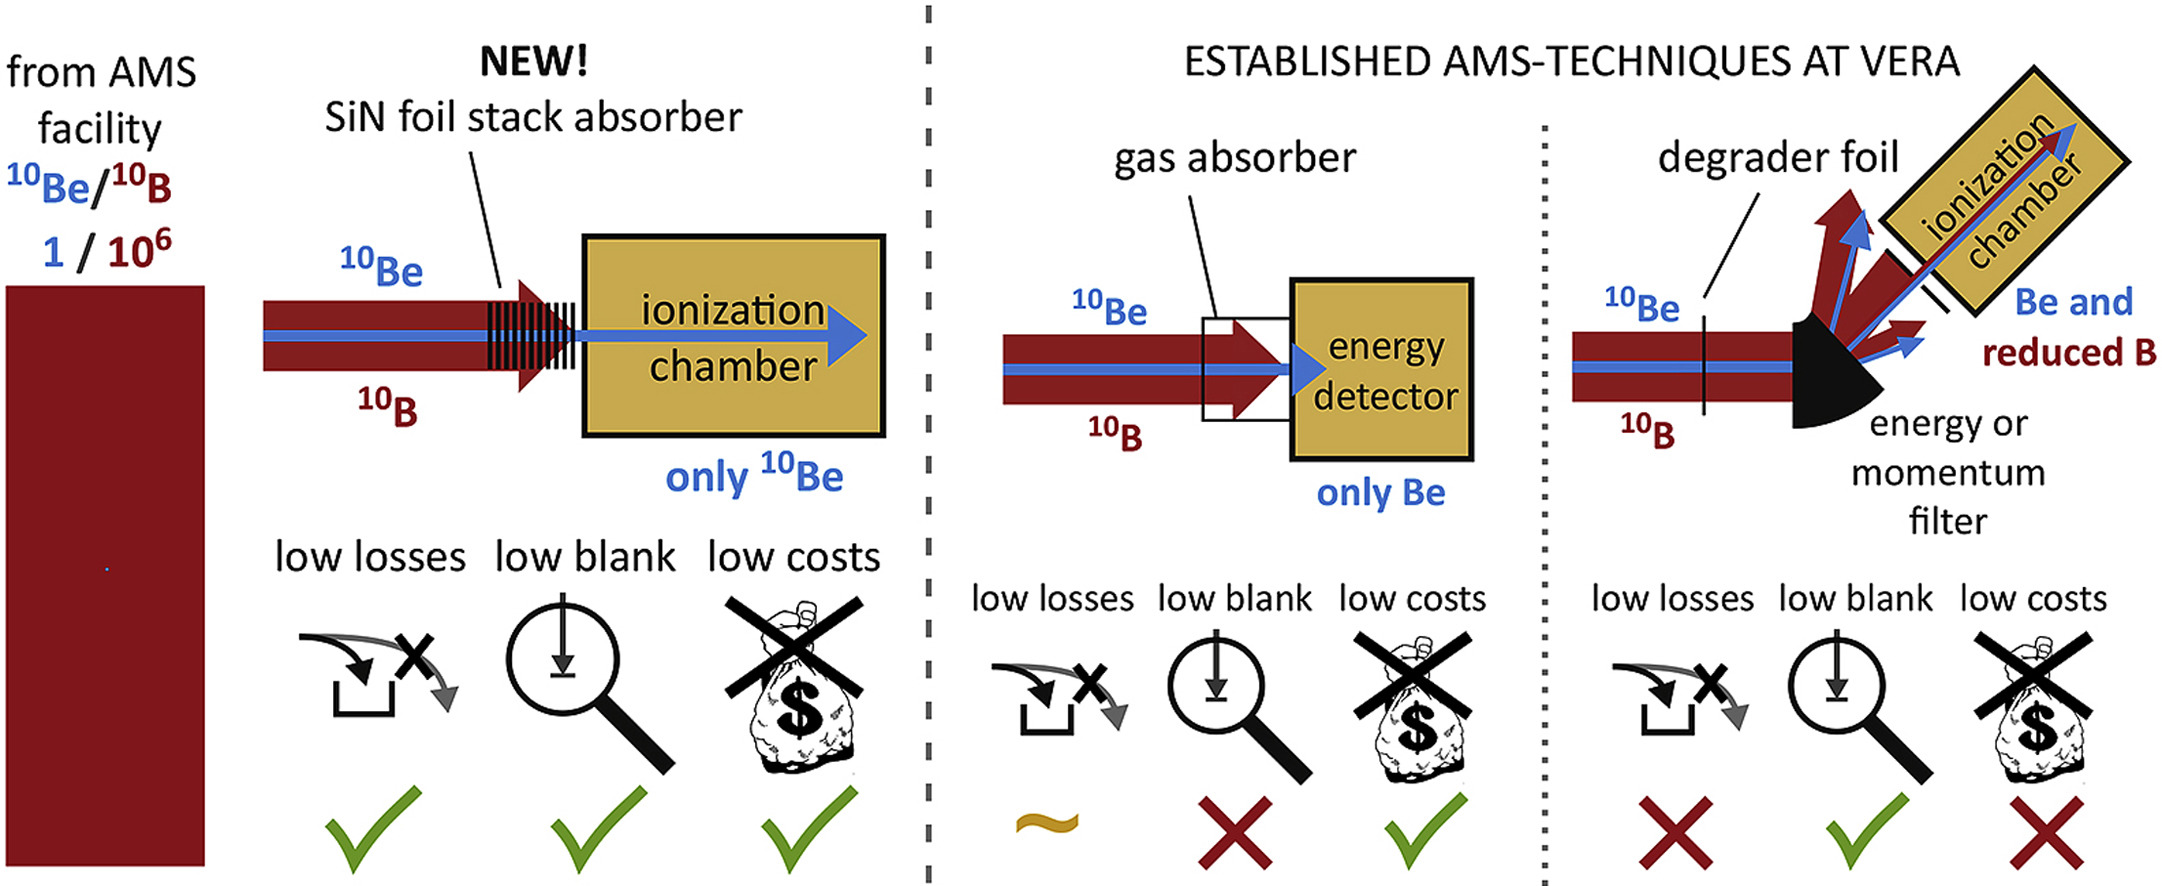
\includegraphics[width=1\linewidth]{B/Generalideaofspecialtheiss.jpg}
    \caption{Comparison of separation methods in AMS, highlighting the new \ce{SiN} foil stack absorber technique from Ref \cite{steier2019}.}
    \label{fig:enter-label}
\end{figure}


By using a composite silicon nitride (\ce{SiN}) foil stack, they have demonstrated an effective way to separate \ce{^{10}Be} from \ce{^{10}B} at higher acceleration potentials. This thesis aims to explore whether this method can be applied at lower voltage settings (1$\MV$), making it feasible for smaller AMS facilities, such as AARAMS. If successful, this technique could improve both the efficiency and accuracy of \ce{^{10}Be} analysis, broadening the accessibility of high-precision dating methods to more laboratories around the world.


\section{Theisis Structure}
The necessary theoretical framework will be introduced, including some sections that are more relevant to this thesis's motivation and the understanding of the setup for the suppression of \ce{^{10}B} in \ce{^{10}Be} AMS measurements.

The experiment's methodology will be introduced, explaining the setups used for the experiments, the corresponding procedures, and the necessary framework for the SRIM simulations, which will be employed to model ion interactions and predict the stopping power and range of ions in the materials involved.

The analysis and discussion will then focus on the experimental results and the general efficiency of the two experimental setups, as well as a proof of concept for the suppression of \ce{^{10}B} using \ce{SiN} stack foils.

Finally, the analysis and discussion will be summarized.
\newpage